\section{Length-Weighting Derivation}
\label{app:normalization}

Fix a rollout batch, its valid-token masks, and domain weights $\lambda_d$. Any PG coefficients are detached. For $n_d=|\mathcal B_d|$, let $\bar T_d=n_d^{-1}\sum_{i\in\mathcal B_d}T_i$ and $\bar g_d=n_d^{-1}\sum_{i\in\mathcal B_d}g_i$. Define the empirical covariance using the same $1/n_d$ normalization:
\begin{equation}
\operatorname{Cov}_d(T,g)=\frac{1}{n_d}\sum_{i\in\mathcal B_d}(T_i-\bar T_d)(g_i-\bar g_d).
\end{equation}
Expanding gives $n_d^{-1}\sum_iT_i g_i-\bar T_d\bar g_d$. Dividing by $\bar T_d$ yields Equation~\ref{eq:weighting}. GT combines the resulting domain gradients using observed token shares; DT combines them using $\lambda_d$; DR combines $\bar g_d$ using $\lambda_d$. Multiplying each domain's globally averaged terms by its target weight divided by its observed token share therefore gives DT exactly.

The derivation is a finite-batch weighted-average identity. Response sampling, masks, and lengths are held fixed. Its population analogue involves an expectation of a ratio; replacing that expectation by a ratio of expectations requires additional assumptions or a large-batch limit.

\subsection{Fixed-batch gradient comparison}
\label{app:fixed_batch_normalization}

At M-PG checkpoints 100 and 250, three banks (seeds 1042, 1043, and 1044) each contain eight responses per domain. Responses use the training prompt format and 4,096-token response cap. For each bank, we compute each response's mean I64 gradient once at the saved BF16 model values using FP32 computation, then aggregate those gradients under DR, DT, and GT. All three reductions use the same responses, token masks, teacher scores, and model coordinates. Student and optimizer snapshots match within each checkpoint.

Table~\ref{tab:fixed_batch_normalization} reports every pairwise raw-gradient cosine. The domain-wise covariance decomposition is checked in FP64 over all 24 bank-domain groups; the largest relative residual is $1.53\times10^{-15}$. This numerical check verifies the aggregation identity. The observed gradient directions establish that the covariance contribution is nonzero on these batches.

The optimizer interventions in Figure~\ref{fig:normalization_interventions} reuse these six banks. Each aggregate gradient is globally clipped at norm 1 and applied to the same saved FP32 Adam state for that bank. The saved-state branch retains both moments; the reset-$m$ branch zeros the first moment while retaining the second moment and optimizer clock; reset-$(m,v)$ zeros both moments while retaining the clock. The momentum-free SGD control follows the negative gradient and is rescaled separately for DR, DT, and GT to match that reduction's saved-state Adam FP32 step norm. Every proposed FP32 step is cast to BF16 before evaluating one held-out response per domain. We report full-vocabulary reverse KL for evaluation; the training-consistent I64 surrogate is retained in the source bundle. These are immediate local interventions, not additional online training runs.

\begin{table}[t]
\caption{Fixed-batch averaging comparison. Entries are raw-gradient cosines; each row uses one shared student and response bank. DR and DT share domain weights and differ only in within-domain response weighting.}
\label{tab:fixed_batch_normalization}
\centering\small
\begin{tabular}{rrrrr}
\toprule
Updates & Batch & DR--DT & DR--GT & DT--GT \\
\midrule
100 & 1 & 0.7838 & 0.6219 & 0.9266 \\
100 & 2 & 0.9110 & 0.5180 & 0.7010 \\
100 & 3 & 0.5780 & 0.6659 & 0.9745 \\
250 & 1 & 0.6240 & 0.4072 & 0.8742 \\
250 & 2 & 0.7864 & 0.3302 & 0.4953 \\
250 & 3 & 0.3990 & 0.3569 & 0.9612 \\
\bottomrule
\end{tabular}

\end{table}

\section{Parameter and Optimizer Measurements}
\label{app:records}

\subsection{Coordinates and recorded quantities}

The online record distinguishes raw aggregate gradients, clipped gradients, actual FP32 optimizer steps, cumulative FP32 master changes, and cumulative BF16 model changes. Cumulative changes use the same initialization reference. All global statistics use unique model coordinates, excluding vocabulary padding and shared duplicates. Per-layer statistics and absolute-threshold sensitivities are retained in the frozen measurements. The sparsity value is the fraction at or below a threshold; figures report its complement. Energy concentration uses squared Euclidean norm and ranks coordinates by absolute change.

For local calculations, the exported checkpoint contains FP32 master values, BF16 model values, first and second moments, optimizer hyperparameters, and step clocks. Student and teacher values are verified against their saved models in the same precision. Local forward/backward computations evaluate these values in FP32 with TF32 disabled. All proposed steps are computed from the same saved state with a non-fused Adam implementation. The online training optimizer uses its own fused implementation.

We evaluate three local states. \emph{Saved} retains both moments and the step clock. \emph{Reset m} zeros the first moment while retaining the second moment and clock. \emph{Fresh} zeros both moments and resets the clock. Global norm clipping at 1 is applied before the Adam calculation, and weight decay is zero. The plotted controls use two response banks; the zero-gradient control is evaluated once. For the zero-gradient branch, the saved first moment continues to decay and move the master weights. A no-step master-to-BF16 cast gives an exact match to the saved model. Figure~\ref{fig:thresholds} shows how absolute thresholds change the measured local activity.

The zero-current-gradient branch changes 0.1403\% of BF16 coordinates, compared with 0.1486\% for PG. Resetting the first moment gives 0.0504\% for PG; resetting both moments and the clock gives 0.5140\%. These controls explain why a sparse gradient selection cannot by itself identify the parameters changed by an optimizer step. They supplement the update-sparsity measurements in Sections~\ref{sec:subnetworks} and~\ref{sec:density}.

Figure~\ref{fig:sampling_history_controls}(b,c) displays these BF16 controls. The full FP32 and BF16 measurements are retained in the evidence bundle.

\begin{figure}[t]
\centering
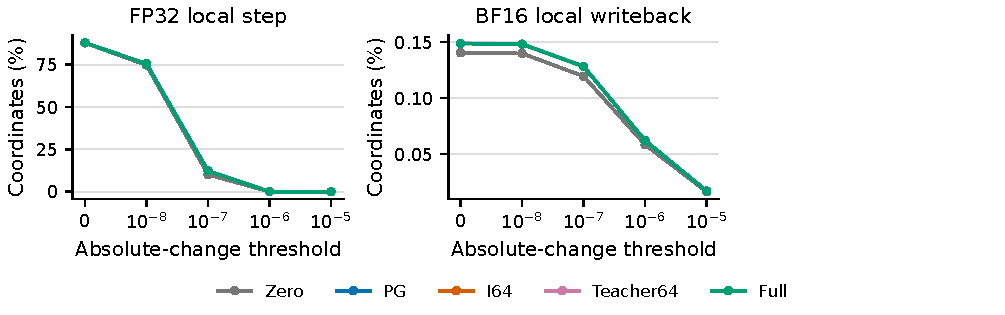
\includegraphics[width=\linewidth]{figures/aligned_evidence_20260910/thresholds.pdf}
\caption{Threshold sensitivity of FP32 steps and BF16 changes. Lines show bank means; shading spans their range.}
\label{fig:thresholds}
\end{figure}

\subsection{Response banks, overlaps, and gradient magnitudes}
\label{app:gradient_overlap}

These raw-gradient diagnostics use the M-PG/100 student, whereas Figure~\ref{fig:subnetwork_overview}(b,c) measures teacher-conditioned optimizer steps at M-PG/500. Banks use seeds 42 and 43, one response per domain per bank, a 2,048-token prompt cap, and a 256-token generation cap. All eight responses reach the cap. Four response positions are sampled without replacement per response. Each row's four prefixes receive equal weight. For routed gradients, each teacher scores its domain row; for common-bank gradients, it scores all four rows with equal domain weights. Crossed comparisons score every domain row with every teacher, keeping the number of prefixes per gradient at four. Crossed and routed/common comparisons share underlying gradients and form paired conditions within banks.

Top-$k$ coordinate sets rank absolute gradient values, using a stable coordinate index to break cutoff ties. Table~\ref{tab:coverage_mass} supplies the routed PG norms; the first bank's instruction-following gradient has norm $1.53\times10^{-9}$. Cosine normalizes magnitude, so opposite directions for such a row carry very little absolute gradient mass. Jaccard overlap measures selected locations and cosine measures signed direction. For reference, independent uniform sets of fraction $\rho$ have expected-intersection to expected-union ratio $\rho/(2-\rho)$, or approximately 0.00503 at $\rho=1\%$. This reference uses uniform coordinates; layer and weight-magnitude structure remain in the measured gradients.

Applying Equation~\ref{subnet_overlap} to the largest-magnitude 1\% of raw-gradient coordinates gives mean routed Jaccard overlaps of 0.0951 for PG and 0.0999 for I64 across the two banks and six teacher pairs. Their ranges are 0.0744--0.1077 and 0.0737--0.1178. When every teacher instead scores all four domain responses, the respective means are 0.3808 and 0.4577. The latter comparison changes both input composition and prefix count; the crossed input control below fixes the count.

Holding the teacher fixed while changing the input domain yields mean gradient cosines of 0.0059 for PG and 0.0072 for I64. Holding the input domain fixed while changing teachers produces both aligned and opposed gradients. For routed gradients the mean cosines are $-0.0020$ and $0.0081$, respectively, despite partial coordinate overlap. Figure~\ref{fig:teacher} supplies this input and direction context for the teacher-overlap results in Section~\ref{sec:subnetworks}.

\begin{figure}[t]
\centering
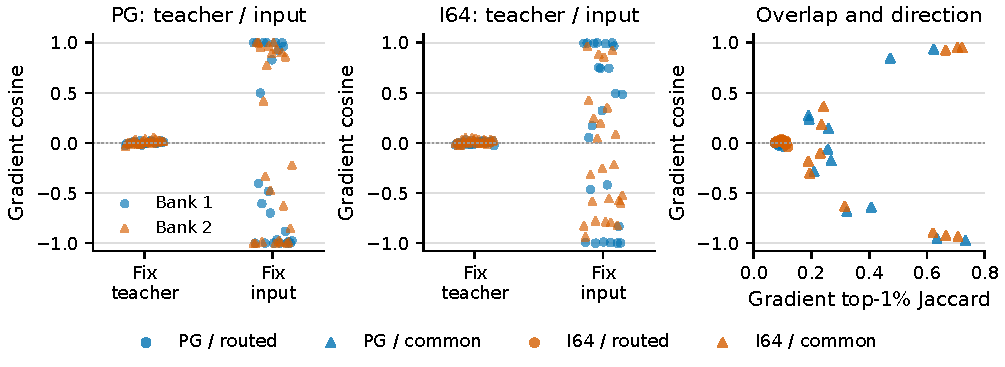
\includegraphics[width=\linewidth]{figures/aligned_evidence_20260910/teacher_input.pdf}
\caption{Input dependence of teacher overlap. Left/center: crossed teacher--input comparisons. Right: top-1\% gradient Jaccard versus signed cosine for routed and common inputs.}
\label{fig:teacher}
\end{figure}

\section{Vocabulary Supervision and Coverage}
\label{app:losses}

\paragraph{Four-bank local experiment.}
The M-PG/100 row of Figure~\ref{fig:supervision_overview}(a) uses four response banks with seeds 2042--2045. Each bank contains one response per domain. Generation uses the training prompt format, a 2,048-token prompt cap, and a 4,096-token response cap. The 16 response lengths range from 81 to 4,096 tokens; two responses reach the cap. Six positions per response give 96 prefixes. PG actions are freshly sampled from the student at the cached prefixes. Every loss uses the same prefixes and domain-response weights. Gradients are globally clipped at norm 1 before applying the same saved Adam state. Table~\ref{tab:local_concentration} adds the FP32 and energy-concentration measurements for this state.

\begin{table}[t]
\centering\small
\caption{Local concentration at M-PG/100, averaged over four matched banks. NZ is the percentage of nonzero coordinates; top-1\% is the percentage of squared step norm carried by the largest 1\% of coordinates. These are local bank means, not training-seed estimates.}
\label{tab:local_concentration}
\begin{tabular}{lrrrr}
\toprule
Loss & FP32 NZ & BF16 NZ & FP32 top-1\% & BF16 top-1\% \\
\midrule
PG & 87.982 & 0.149 & 8.845 & 100.000 \\
I64 & 87.989 & 0.150 & 8.827 & 100.000 \\
T64 & 87.989 & 0.150 & 8.828 & 100.000 \\
Full & 87.999 & 0.150 & 8.828 & 100.000 \\
\bottomrule
\end{tabular}

\end{table}

The local loss and Adam implementations are the same as in the two-bank controls in Appendix~\ref{app:records}. Appendix~\ref{app:actual_intersection_coverage} reports the actual I64 intersection coverage across all four student states.


\paragraph{Implementation details.}
For I64 (Equation~\ref{eq:topk}), candidate sets and teacher scores are fixed at rollout. Each student forward recomputes current probabilities at the saved candidate positions and refreshes the detached coefficients. PG also refreshes its detached log-ratio coefficients and uses no advantage or policy-ratio clipping.

\paragraph{Teacher-top-64 local reference.}
The teacher-top-64 diagnostic uses the fixed teacher set $T$ and full-vocabulary probabilities:
\begin{equation}
\ell_{\mathrm{T64}}=\sum_{v\in T}\left[p_\theta(v)\log\frac{p_\theta(v)}{q_d(v)}-p_\theta(v)+q_d(v)\right].
\label{eq:t64}
\end{equation}
Its gradient is $\sum_{v\in T}p_\theta(v)\log(p_\theta(v)/q_d(v))\nabla_\theta\log p_\theta(v)$. I64 instead uses the detached weights in Equation~\ref{eq:topk}, normalized over the original student set $S$. T64 and full vocabulary are local objective comparisons; online capability curves compare PG, I16, and I64. I16 has no corresponding local geometry measurement.

For a fixed prefix, differentiating Equation~\ref{eq:full} gives
\begin{align}
\nabla_\theta\ell_{\mathrm{full}}
&=\sum_{v\in\cV}p_\theta(v)\left(\log\frac{p_\theta(v)}{q_d(v)}+1\right)\nabla_\theta\log p_\theta(v)\\
&=\mathbb E_{a\sim p_\theta}\!\left[\log\frac{p_\theta(a)}{q_d(a)}\nabla_\theta\log p_\theta(a)\right],
\end{align}
using $\sum_v\nabla_\theta p_\theta(v)=0$. The identity conditions on prefixes and fixed weights. Original rollout losses additionally use the realized response and its eventual length-dependent weight. Table~\ref{tab:coverage_mass} reports the corresponding coverage for the two-bank controls used to interpret gradient overlap and optimizer history.

\begin{table}[t]
\caption{Teacher-top-64 coverage and routed gradient scale in the two-bank controls. Probability mass and student entropy (nats) are prefix averages; displayed 100\% values may reflect rounding.}
\label{tab:coverage_mass}
\centering\small
\begin{tabular}{rlrrrr}
\toprule
Bank & Domain & Mass in $T$ (\%) & Mass in $I$ (\%) & Entropy & $\|g_{\mathrm{PG}}\|_2$ \\
\midrule
1 & Math & 100.0000 & 100.0000 & 0.3243 & 132.6 \\
1 & Code & 99.9968 & 99.9965 & 0.7701 & 163.8 \\
1 & IF & 100.0000 & 100.0000 & $1.85\times10^{-5}$ & $6.13\times10^{-9}$ \\
1 & Science & 99.9184 & 99.9162 & 0.7405 & 54.82 \\
2 & Math & 99.9991 & 99.9991 & 0.3221 & 2.605 \\
2 & Code & 100.0000 & 100.0000 & 0.2962 & 3.167 \\
2 & IF & 100.0000 & 100.0000 & 0.5004 & 55.52 \\
2 & Science & 99.9993 & 99.9992 & 0.2442 & 0.8505 \\
\bottomrule
\end{tabular}

\end{table}

\section{Teacher Distribution Distance}
\label{app:teacher_distance}

Teacher distance is computed on the full next-token vocabulary at matched prefixes:
\begin{equation}
\operatorname{JS}(q_d,q_e)=\tfrac12 D_{\mathrm{KL}}(q_d\|m)+\tfrac12 D_{\mathrm{KL}}(q_e\|m),
\qquad m=\tfrac12(q_d+q_e).
\label{eq:teacher_js}
\end{equation}
We average over the same equally weighted domains and prefixes for every pair. Figure~\ref{fig:teacher_overlap_support}(b) pairs this distance with common-input optimizer-step selections at M-PG/500. The earlier M-PG/100 raw-gradient diagnostic contains twelve bank-pair JS measurements, ranging from 0.00151 to 0.02714 nats; its pair-level records remain in the evidence bundle. Both diagnostics share teachers and prefixes within each bank, so teacher-pair observations are dependent.
